\section{Analisis Pengujian Sudut Pandang Kamera}
\label{sec:analisis_sudutkamera}

\par Dilakukan pengujian model dan sistem pada sudut pandang yang berbeda antara objek yang diamati (orang) dan kamera. Pada pengujian ini peletakan kamera dengan arah berbeda sulit dilakukan, maka dari itu digantikan dengan mengubah arah pandang personel/orang yang sedang diamati. 

\begin{table}
    \centering
    \caption{Hasil Pengujian Model Pada Sudut Pandang Kamera Berbeda}
    \label{tb:analisis_model_diffarah}
    \begin{tabular}{|l|l|l|l|l|l|l|l|} 
    \hline
    Arah                                & Kelas           & TP & TN & FP & FN & Precision    & Recall        \\ 
    \hline
    \multirow{3}{*}{Menghadap (0)}      & with\_helmet    & 11 &    & 5  & 0  & 0.6875       & 1             \\ 
    \cline{2-8}
                                        & no\_helmet      & 14 &    & 0  & 5  & 1            & 0.7368421053  \\ 
    \cline{2-8}
                                        & all (rata-rata) &    &    &    &    & 0.84375      & 0.8684210526  \\ 
    \hline
    \multirow{3}{*}{Membelakangi (180)} & with\_helmet    & 10 &    & 2  & 0  & 0.8333333333 & 1             \\ 
    \cline{2-8}
                                        & no\_helmet      & 12 &    & 0  & 3  & 1            & 0.8           \\ 
    \cline{2-8}
                                        & all (rata-rata) &    &    &    &    & 0.9166666667 & 0.9           \\ 
    \hline
    \multirow{3}{*}{Kanan (90)}         & with\_helmet    & 6  &    & 8  & 0  & 0.4285714286 & 1             \\ 
    \cline{2-8}
                                        & no\_helmet      & 10 &    & 0  & 3  & 1            & 0.7692307692  \\ 
    \cline{2-8}
                                        & all (rata-rata) &    &    &    &    & 0.7142857143 & 0.8846153846  \\ 
    \hline
    \multirow{3}{*}{Kiri (270)}         & with\_helmet    & 6  &    & 1  & 1  & 0.8571428571 & 0.8571428571  \\ 
    \cline{2-8}
                                        & no\_helmet      & 16 &    & 0  & 2  & 1            & 0.8888888889  \\ 
    \cline{2-8}
                                        & all (rata-rata) &    &    &    &    & 0.9285714286 & 0.873015873   \\
    \hline
    \end{tabular}
\end{table}

\par Berdasarkan hasil pengujian model yang ditunjukan pada Tabel~\ref{tb:analisis_model_diffarah}, ditemukan beberapa poin analisa. Pada umumnya, \emph{True Positive} dari kelas "with\_helmet" maupun "no\_helmet" daripada \emph{False Positive} ataupun \emph{False Negative} nya seperti yang ditunjukan pada Gambar~\ref{fig:example_true_direct}. Hasil presisi rata-rata paling buruk terdapat pada arah menghadap ke kanan (90 derajat) dimana nilai \emph{precision}nya 0.71 dimana pada arah ini nilai \emph{precision} dari kelas "with\_helmet" bernilai 0.43 karena sering terjadi \emph{False Positive} seperti yang ditunjukkan pada Gambar~\ref{fig:example_fp_direct_right}. Kelas "no\_helmet" umumnya mengalami \emph{False Negative} pada semua arah dari 1 kali hingga 5 kali seperti yang ditunjukkan pada Gambar~\ref{fig:example_fn_nohelm_all}. 

\begin{table}
    \centering
    \caption{Hasil Pengujian Sistem Deteksi Pada Sudut Pandang Kamera Berbeda}
    \label{tb:analisis_sys_diffarah}
    \begin{tabular}{|l|l|l|l|l|l|l|} 
    \hline
    Arah               & Jumlah Tes & TP & TN & FP & FN & Akurasi       \\ 
    \hline
    Menghadap (0)      & 30         & 14 & 11 & 0  & 5  & 0.8333333333  \\ 
    \hline
    Membelakangi (180) & 25         & 12 & 10 & 0  & 3  & 0.88          \\ 
    \hline
    Kanan (90)         & 22         & 10 & 7  & 0  & 5  & 0.7727272727  \\ 
    \hline
    Kiri (270)         & 25         & 16 & 7  & 0  & 2  & 0.92          \\
    \hline
    \end{tabular}
\end{table}

\par Pada pengujian sistem yang ditunjukan pada Tabel~\ref{tb:analisis_sys_diffarah}, ditarik beberapa poin analisis. Seperti pada analisis model, arah hadap Kanan (90) memiliki nilai akurasi paling rendah dibanding arah lainnya yaitu 0.77 dimana dari 25 kali pengambilan sampel pengujian, 5 kali mengalami \emph{False Negative}.

\begin{figure} [h]
    \centering
    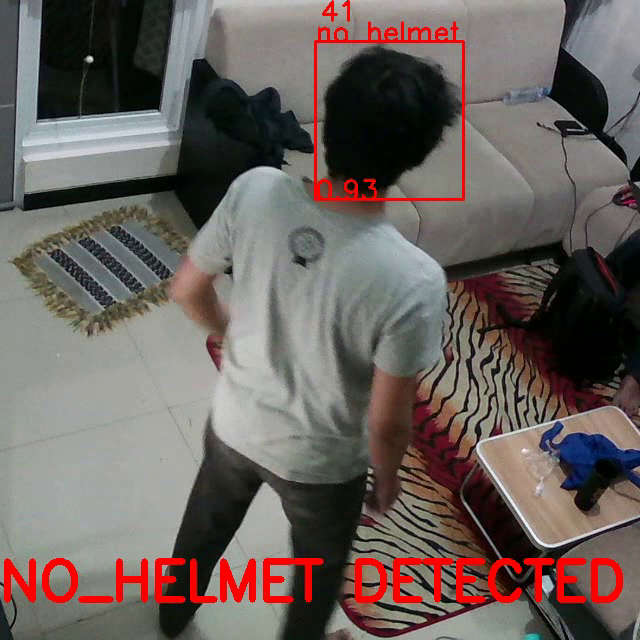
\includegraphics[width=0.24\textwidth]{gambar/analisis_gambar/contoh_betul/test1_cctv_pred (6).png}
    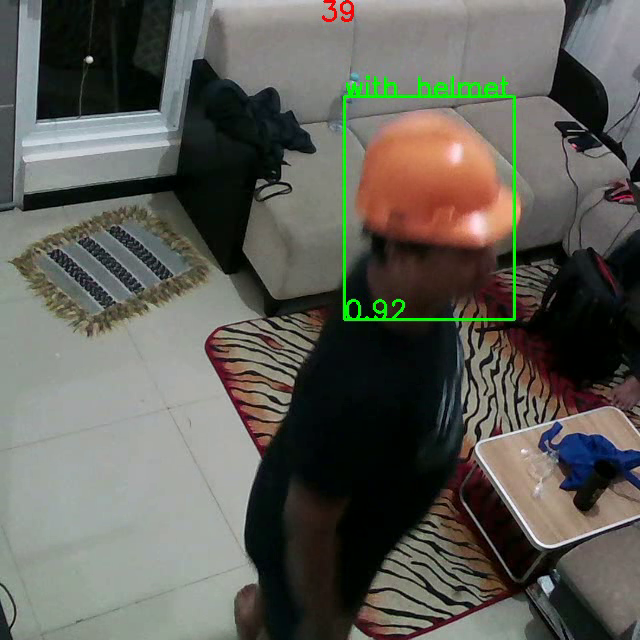
\includegraphics[width=0.24\textwidth]{gambar/analisis_gambar/contoh_betul/test2_cctv_pred (14).png}
    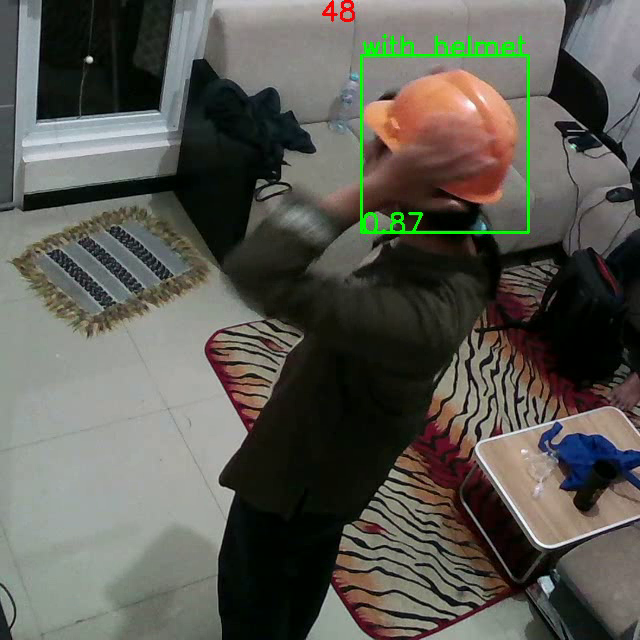
\includegraphics[width=0.24\textwidth]{gambar/analisis_gambar/contoh_betul/test3_cctv_pred (15).png}
    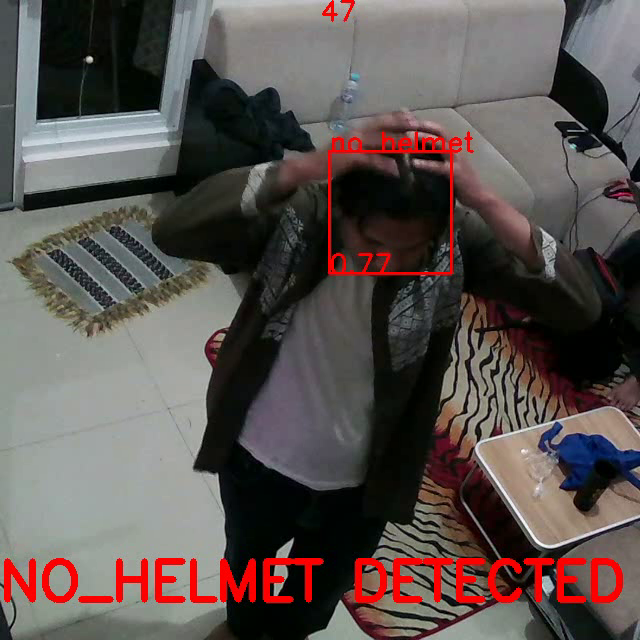
\includegraphics[width=0.24\textwidth]{gambar/analisis_gambar/contoh_betul/test3_cctv_pred (3).png}
    \caption{Contoh Deteksi \emph{True} Pada Perbedaan Sudut Pandang}
    \label{fig:example_true_direct}  
\end{figure}

\begin{figure} [h]
    \centering
    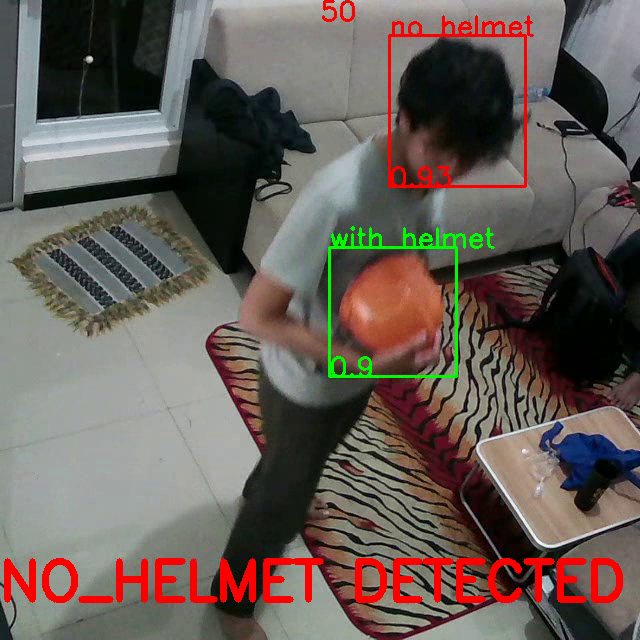
\includegraphics[width=0.3\textwidth]{gambar/analisis_gambar/kanan_salah_FPhelm/test1_cctv_pred (12).png}
    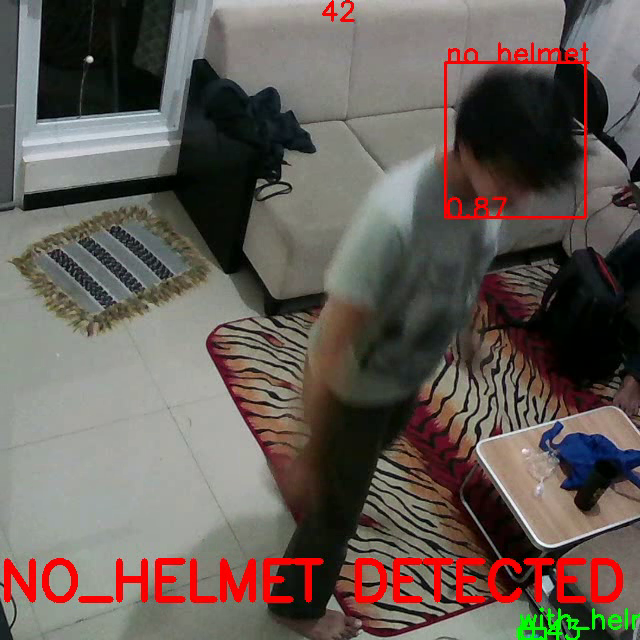
\includegraphics[width=0.3\textwidth]{gambar/analisis_gambar/kanan_salah_FPhelm/test1_cctv_pred.png}
    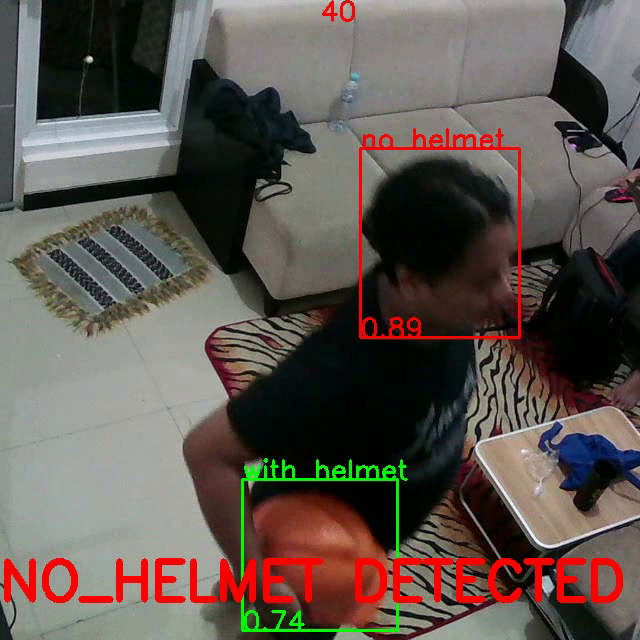
\includegraphics[width=0.3\textwidth]{gambar/analisis_gambar/kanan_salah_FPhelm/test2_cctv_pred (10).png}
    \caption{Contoh Deteksi \emph{False Positive} Kelas "with\_helmet" Pada Arah Kanan (90 derajat)}
    \label{fig:example_fp_direct_right}
\end{figure}

\begin{figure} [h]
    \centering
    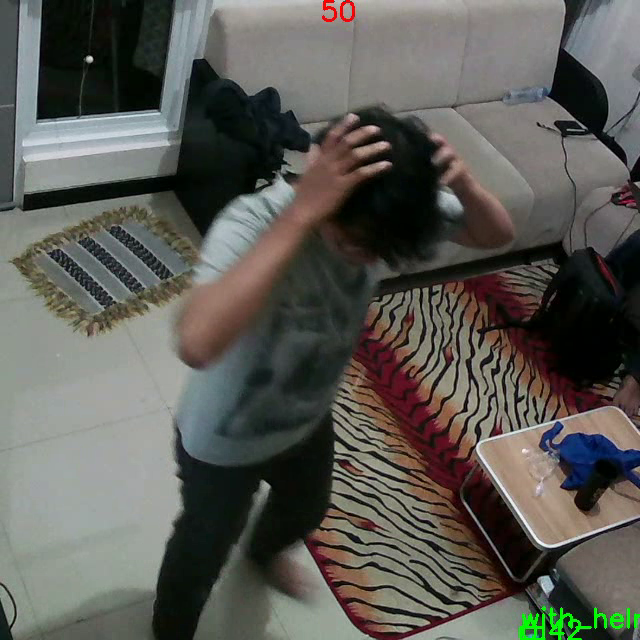
\includegraphics[width=0.3\textwidth]{gambar/analisis_gambar/semua_salah_FNno/test1_cctv_pred (6).png}
    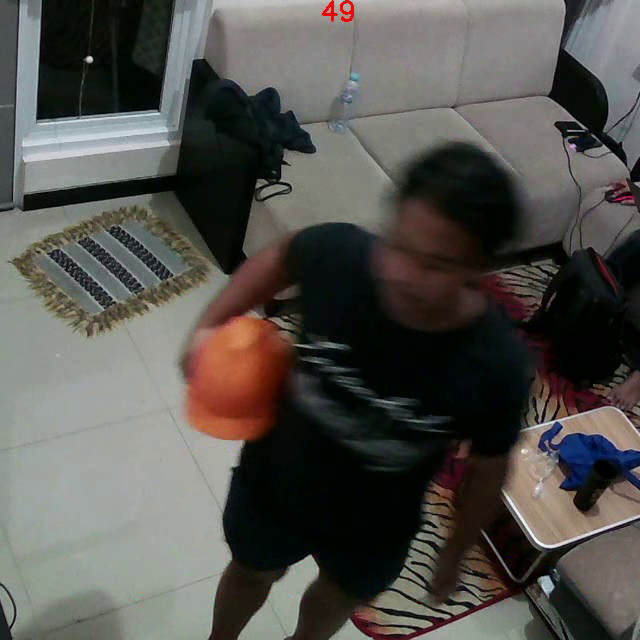
\includegraphics[width=0.3\textwidth]{gambar/analisis_gambar/semua_salah_FNno/test2_cctv_pred (18).png}
    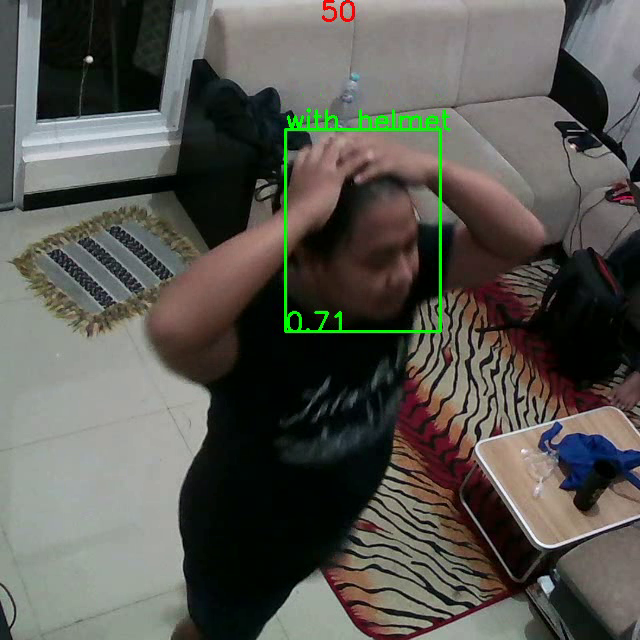
\includegraphics[width=0.3\textwidth]{gambar/analisis_gambar/semua_salah_FNno/test2_cctv_pred (4).png}
    \caption{Contoh Deteksi \emph{False Negative} Kelas "no\_helmet" Pada Perbedaan Sudut Pandang}
    \label{fig:example_fn_nohelm_all}
\end{figure}